% Process-flow diagram of the audit-and-compensate procedure (black and white).
% Compile with pdflatex to obtain fig_flow.pdf, which the main paper includes.
\documentclass[tikz,border=4pt]{standalone}
\usepackage{amsmath,amssymb}
\usetikzlibrary{arrows.meta,positioning,shapes.geometric,fit}
\begin{document}
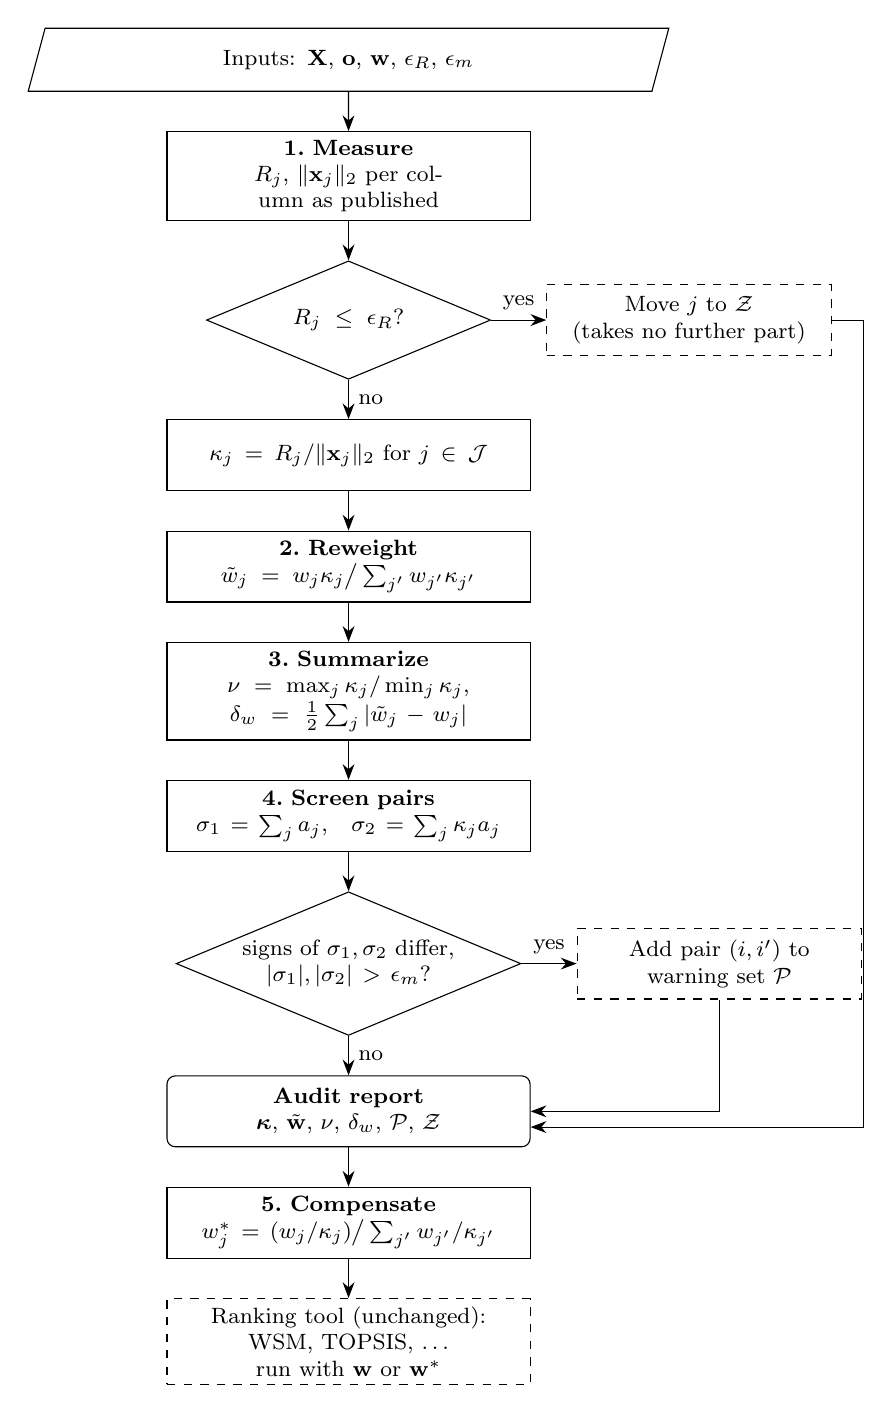
\begin{tikzpicture}[font=\footnotesize, >={Stealth[length=2mm]}, node distance=5mm and 7mm,
  io/.style={draw, trapezium, trapezium left angle=75, trapezium right angle=105, minimum height=8mm, text width=36mm, align=center, inner sep=2pt},
  proc/.style={draw, rectangle, minimum height=9mm, text width=44mm, align=center, inner sep=3pt},
  dec/.style={draw, diamond, aspect=2.4, text width=27mm, align=center, inner sep=1pt},
  outp/.style={draw, rectangle, rounded corners=3pt, minimum height=9mm, text width=44mm, align=center, inner sep=3pt},
  side/.style={draw, dashed, rectangle, minimum height=9mm, text width=34mm, align=center, inner sep=3pt}]
\node[io] (in) {Inputs: $\mathbf{X}$, $\mathbf{o}$, $\mathbf{w}$, $\epsilon_R$, $\epsilon_m$};
\node[proc, below=of in] (s1) {\textbf{1.\ Measure}\\ $R_j$, $\|\mathbf{x}_j\|_2$ per column as published};
\node[dec, below=of s1] (d1) {$R_j\le\epsilon_R$?};
\node[side, right=of d1] (z) {Move $j$ to $\mathcal{Z}$\\ (takes no further part)};
\node[proc, below=of d1] (s1b) {$\kappa_j=R_j/\|\mathbf{x}_j\|_2$ for $j\in\mathcal{J}$};
\node[proc, below=of s1b] (s2) {\textbf{2.\ Reweight}\\ $\tilde w_j=w_j\kappa_j\big/\sum_{j'}w_{j'}\kappa_{j'}$};
\node[proc, below=of s2] (s3) {\textbf{3.\ Summarize}\\ $\nu=\max_j\kappa_j/\min_j\kappa_j$,\quad $\delta_w=\tfrac12\sum_j|\tilde w_j-w_j|$};
\node[proc, below=of s3] (s4) {\textbf{4.\ Screen pairs}\\ $\sigma_1=\sum_j a_j$,\quad $\sigma_2=\sum_j\kappa_j a_j$};
\node[dec, below=of s4] (d2) {signs of $\sigma_1,\sigma_2$ differ, $|\sigma_1|,|\sigma_2|>\epsilon_m$?};
\node[side, right=of d2] (p) {Add pair $(i,i')$ to\\ warning set $\mathcal{P}$};
\node[outp, below=of d2] (out) {\textbf{Audit report}\\ $\boldsymbol{\kappa}$, $\tilde{\mathbf{w}}$, $\nu$, $\delta_w$, $\mathcal{P}$, $\mathcal{Z}$};
\node[proc, below=of out] (s5) {\textbf{5.\ Compensate}\\ $w^{*}_j=(w_j/\kappa_j)\big/\sum_{j'}w_{j'}/\kappa_{j'}$};
\node[side, below=of s5, text width=44mm] (rank) {Ranking tool (unchanged):\\ WSM, TOPSIS, \dots\ run with $\mathbf{w}$ or $\mathbf{w}^{*}$};
\draw[->] (in)--(s1); \draw[->] (s1)--(d1); \draw[->] (d1)--node[above]{yes}(z); \draw[->] (d1)--node[right]{no}(s1b);
\draw[->] (s1b)--(s2); \draw[->] (s2)--(s3); \draw[->] (s3)--(s4); \draw[->] (s4)--(d2);
\draw[->] (d2)--node[above]{yes}(p); \draw[->] (d2)--node[right]{no}(out); \draw[->] (p)|-(out);
\draw[->] (z.east) -- ++(4mm,0) |- ([yshift=-2mm]out.east);
\draw[->] (out)--(s5); \draw[->] (s5)--(rank);
\end{tikzpicture}
\end{document}
